\documentclass[spanish, fleqn]{article}
\usepackage{babel}
\usepackage[utf8]{inputenc}
\usepackage{amsmath,amsfonts}
\usepackage{enumitem}
\usepackage[colorlinks, urlcolor=blue]{hyperref}
\usepackage{fourier}
\usepackage[top = 2.5cm, bottom = 2cm, left = 2.5cm, right = 2.5cm]{geometry}
\usepackage{tikz}
\usetikzlibrary{positioning,arrows}
\usepackage{pgf}
\usepackage{color}


\title{Estructuras Discretas \\
       Actividad Extra \#2 \\
       ``Grafos''}
\author{Alondra Rojas Ruz}
\date{02 de junio, 2017}

\begin{document}
\maketitle
\thispagestyle{empty}

%Esta actividad es optativa y quienes la realicen pueden optar hasta 5 puntos en el certamen 1. Es un complemento a lo visto en clases sobre inducción.

\section*{Instrucciones}

\begin{itemize}
    \item Lea atentamente desde la sección \textbf{24.1} hasta la sección \textbf{24.5} del capítulo 4 \href{https://moodle.inf.utfsm.cl/pluginfile.php?file=\%2F64673\%2Fmod_resource\%2Fcontent\%2F2\%2Fclases-0.83.pdf}{apunte} del curso, encontrado en la sección \textbf{material de clases}. Asegúrese de entender los conceptos principales relacionados a la teoría de grafos, para luego discutirlos en clases.
    \item Puede complementarlo con investigación propia.
    \item A partir de su lectura responda las siguientes preguntas (todas deben estar correctamente justificadas):
    
\end{itemize}
    
\section*{Preguntas}
    
\begin{enumerate}
\item Busque y mencione dos ejemplos prácticos donde se utilicen grafos en problemas de la computación.

Dado que los grafos en la computación se usan para representar de forma cómoda relaciones entre objetos,podemos dar como ejemplo el uso de estos para la representación de una red de transporte, pudiendo ser esta un sistema de metros en donde las relaciones vendrían a ser las conexiones entre las estaciones. Otra aplicación de estos podria ser su uso en problemas de optimización para establecer conexiones más directas entre objetos.

\hspace*{\fill}(1 punto)  
\item Escriba la definición formal de un grafo y mencione 2 ejemplos indicando que representan los arcos y vértices.

Un grafo consta de un conjunto no vacio de vertices finitos(V) y un conjunto de arcos(E), que corresponden a pares de vertices pertenecientes a V. 

Grafo de relaciones amorosas, en donde los vertices representan a las personas y los arcos, a si estos se han relacionado amorosamente.

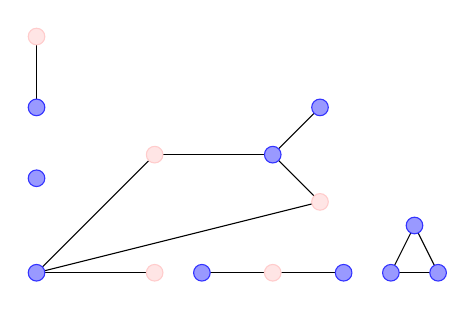
\begin{tikzpicture}[y=.3cm, x=.3cm,font=\normalsize]
\draw (0,0) -- (5,5);
\draw (5,5) -- (10,5);
\draw (0,0) -- (5,0);
\draw (10,5) -- (12,7);
\draw (10,5) -- (12, 3);
\draw (0,0) -- (12, 3);
\draw (0,7) -- (0,10);
\draw (0,4);
\draw (7,0) -- (10,0);
\draw (13,0) -- (10,0);
\draw (15,0) -- (17,0);
\draw (15,0) --(16,2);
\draw (16,2)--(17,0);


;\filldraw[fill=blue!40,draw=blue!80] (0,0) circle (3pt)  ;
\filldraw[fill=pink!40,draw=pink!80] (5,5) circle (3pt)     ;
\filldraw[fill=pink!40,draw=pink!80] (5,0) circle (3pt)     ;
\filldraw[fill=blue!40,draw=blue!80] (10,5) circle (3pt)     ;
\filldraw[fill=blue!40,draw=blue!80] (12,7) circle (3pt)     ;
\filldraw[fill=pink!40,draw=pink!80] (12,3) circle (3pt)     ;
\filldraw[fill=pink!40,draw=pink!80] (0,10) circle (3pt)     ;
\filldraw[fill=blue!40,draw=blue!80] (0,7) circle (3pt)     ;
\filldraw[fill=blue!40,draw=blue!80] (0,4) circle (3pt)     ;
\filldraw[fill=pink!40,draw=pink!80] (10,0) circle (3pt)     ;
\filldraw[fill=blue!40,draw=blue!80] (7,0) circle (3pt)     ;
\filldraw[fill=blue!40,draw=blue!80] (13,0) circle (3pt)     ;
\filldraw[fill=blue!40,draw=blue!80] (15,0) circle (3pt)     ;
\filldraw[fill=blue!40,draw=blue!80] (17,0) circle (3pt)     ;
\filldraw[fill=blue!40,draw=blue!80] (16,2) circle (3pt)     ;

\end{tikzpicture}

Grafo de paises colindantes, en donde los vertices representan a los paises y los arcos si estos estan uno al lado del otro.

\begin{tikzpicture}[y=.3cm, x=.3cm,font=\normalsize]
\draw (0,0) -- (5,0);
\draw (0,0) -- (0,5);
\draw (0,0) -- (3,3);
\draw (3,3) -- (10,10);
\draw(5,0)--(10,10);
\draw(0,5)--(10,10);
\draw (10,0)--(10,10);
\draw (0,5)--(10,10);
\draw (5,0)--(10,0);
\draw (0,5)--(3,3);
\draw (5,0)--(3,3);
\draw (12,2)--(3,3);
\draw (12,2)--(5,0);
\draw (12,2)--(10,10);

\filldraw[fill=black!40,draw=black!80] (0,0) circle (3pt)   ;
\filldraw[fill=black!40,draw=black!80] (0,5) circle (3pt)    ;
\filldraw[fill=black!40,draw=black!80] (5,0) circle (3pt)    ;
\filldraw[fill=black!40,draw=black!80] (3,3) circle (3pt)  ;
\filldraw[fill=black!40,draw=black!80] (10,10) circle (3pt)  ;
\filldraw[fill=black!40,draw=black!80] (10,0) circle (3pt)  ;
\filldraw[fill=black!40,draw=black!80] (3,3) circle (3pt)  ;
\filldraw[fill=black!40,draw=black!80] (3,3) circle (3pt)  ;
\filldraw[fill=black!40,draw=black!80] (12,2) circle (3pt)  ;

\node [above] at (0,5) {$Perú$};
\node [below] at (0,0) {$Chile$};
\node [right] at (12,2) {$Paraguay$};
\node [right] at (10,0) {$Uruguay$};
\node [above, rotate=45] at (3,3) {$Bolivia$};
\node [below] at (5,0) {$Argentina$};
\node [right][] at (10,10) {$Brasil$};
\end{tikzpicture}

\item Invente un grafo con 10 vértices y represéntelo utilizando \emph{lista de adyacencia}, \emph{matriz de adyacencia} y \emph{gráficamente} y luego dibuje un grafo \emph{isomorfo} al grafo que inventó.

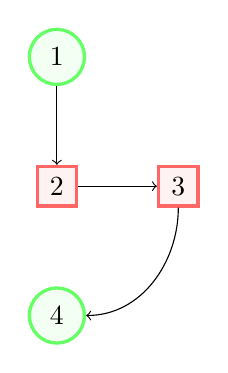
\begin{tikzpicture}[
roundnode/.style={circle, draw=green!60, fill=green!5, very thick, minimum size=7mm},
squarednode/.style={rectangle, draw=red!60, fill=red!5, very thick, minimum size=5mm},
]
%Nodes
\node[squarednode]      (maintopic)                              {2};
\node[roundnode]        (uppercircle)       [above=of maintopic] {1};
\node[squarednode]      (rightsquare)       [right=of maintopic] {3};
\node[roundnode]        (lowercircle)       [below=of maintopic] {4};
 
%Lines
\draw[->] (uppercircle.south) -- (maintopic.north);
\draw[->] (maintopic.east) -- (rightsquare.west);
\draw[->] (rightsquare.south) .. controls +(down:7mm) and +(right:7mm) .. (lowercircle.east);
\end{tikzpicture}

\hspace*{\fill}(2 puntos)  

\item En la sección \textbf{24.4} aparecen algunas familias especiales de grafos, describa \textbf{informalmente}, es decir, con sus propias palabras, de que se trata cada una de ellas.

\hspace*{\fill}(1 punto)  
\end{enumerate}



%% Pregunta 3

  \vfill\hfill ARR/\LaTeXe
\end{document}
